\subsection{DEFINITION OF A UNIFORM STRUCTURE}

DEFINITION 1. A uniform structure (or uniformity) on a set X is a structure given by a set U of subsets of X × X which satisfies axioms (F\_I) and (F\_II) of Chapter I, § 6, no. 1 and also satisfies the following axioms:

\((\mathbf{U}_{\mathbf{I}})\) Every set belonging to \(\mathfrak{U}\) contains the diagonal \(\Delta\) .

\((\mathbf{U}_{\mathbf{II}})\) If \(\mathbf{V}\in \mathfrak{U}\) then \(\overline{\mathbf{V}}^1\in \mathfrak{U}\) .

\((\mathbf{U}_{\mathbf{III}})\) For each \(\mathbf{V} \in \mathfrak{U}\) there exists \(\mathbf{W} \in \mathfrak{U}\) such that \(\mathbf{W} \circ \mathbf{W} \subset \mathbf{V}\) .

\pandocbounded{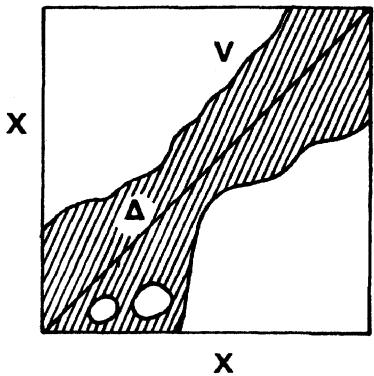
\includegraphics[keepaspectratio]{images/part001_6ce88dc6.jpg}}\\
Figure 2.

The sets of \(\mathfrak{U}\) are called entourages of the uniformity defined on \(\mathbf{X}\) by \(\mathfrak{U}\) . A set endowed with a uniformity is called a uniform space.

If V is an entourage of a uniformity on X, we may express the relation \((x, x') \in V\) by saying that ``x and \(x'\) are V-close''.

Remarks. 1) To make the language more expressive we may use the expressions ``x is close enough to y'' and ``x and y are as close as we please'' in some statements. For example, we shall say that a relation

R \(\{x,y\}\) is true whenever x and y are close enough if there is an entourage V such that the relation \((x,y)\in V\) implies R \(\{x,y\}\) .

\begin{enumerate}
\def\labelenumi{\arabic{enumi})}
\setcounter{enumi}{1}
\tightlist
\item
  The conjunction of axioms (U \(_{II}\) ) and (U \(_{III}\) ) is equivalent (assuming the other axioms of uniform structures) to the following axiom:
\end{enumerate}

\((\mathbf{U}_a)\) For each \(\mathbf{V} \in \mathfrak{U}\) there exists \(\mathbf{W} \in \mathfrak{U}\) such that \(\mathbf{W} \circ \overline{\mathbf{W}} \subset \mathbf{V}\) (*).

Clearly \((\mathbf{U}_{\mathrm{II}})\) and \((\mathbf{U}_{\mathrm{III}})\) imply \((\mathbf{U}_a)\) . Conversely, if \((\mathbf{U}_a)\) is satisfied we have \(\overline{\mathbf{W}} = \Delta \circ \overline{\mathbf{W}} \subset \mathbf{V}\) , by \((\mathbf{U}_I)\) ; hence \(\mathbf{W} \subset \overline{\mathbf{V}}\) and therefore {[}by \((\mathbf{F}_I)] \overline{\mathbf{V}} \in \mathfrak{U}\) . Let \(\mathbf{W}' = \mathbf{W} \cap \overline{\mathbf{W}}\) ; then \(\mathbf{W}' \in \mathfrak{U}\) by what has just been proved and axiom \((\mathbf{F}_{\mathrm{II}})\) , and we have \(\mathbf{W}' \circ \mathbf{W}' \subset \mathbf{W} \circ \overline{\mathbf{W}} \subset \mathbf{V}\) .

Throughout this chapter we shall write \(\mathbf{V}\) instead of \(\mathbf{V} \circ \mathbf{V}\) , and in general \(\mathbf{V} = \mathbf{V} \circ \mathbf{V} = \mathbf{V} \circ \mathbf{V}\) , for each integer \(n > 1\) and each subset \(\mathbf{V}\) of \(\mathbf{X} \times \mathbf{X}\) .

\begin{enumerate}
\def\labelenumi{\arabic{enumi})}
\setcounter{enumi}{2}
\tightlist
\item
  If X is not empty, then axiom \((U_{I})\) implies that no set of U is empty, and therefore U is a filter on \(X \times X\) . There is only one uniformity on the empty set, namely \(U = \{\varnothing\}\) .
\end{enumerate}

DEFINITION 2. A fundamental system of entourages of a uniformity is any set B of entourages such that every entourage contains a set belonging to B.

Axiom \((\mathbf{U}_{\mathbf{III}})\) shows that if n is any integer \textgreater0 and V runs through a fundamental system of entourages, then the sets \(V^{n}\) again form a fundamental system of entourages.

Entourages V such that \(V = \overline{V}^{1}\) are called symmetric. If V is any entourage, then \(V \cap \overline{V}^{1}\) and \(V \cup \overline{V}^{1}\) are symmetric entourages, and axioms \((F_{\mathrm{II}})\) and \((U_{\mathrm{II}})\) show that the symmetric entourages form a fundamental system of entourages.

A set \(\mathfrak{B}\) of subsets of \(\mathbf{X} \times \mathbf{X}\) is a fundamental system of entourages of a uniformity on \(\mathbf{X}\) if and only if \(\mathfrak{B}\) satisfies axiom ( \(B_{\mathbf{I}}\) ) of Chapter I, § 6, no. 3, and also satisfies the following axioms:

\((\mathbf{U}_{\mathbf{I}}^{\prime})\) Every set of \(\mathfrak{B}\) contains the diagonal \(\Delta\) .

\((\mathbf{U}_{\mathbf{II}}^{\prime})\) For each \(\mathbf{V} \in \mathfrak{B}\) there exists \(\mathbf{V}' \in \mathfrak{B}\) such that \(\mathbf{V}' \subset \overline{\mathbf{V}}^1\) .

\((\mathbf{U}_{\mathbf{III}}^{\prime})\) For each \(\mathbf{V} \in \mathfrak{B}\) there exists \(\mathbf{W} \in \mathfrak{B}\) such that \(\tilde{\mathbf{W}} \subset \mathbf{V}\) .

If X is not empty, a fundamental system of entourages of a uniform structure on X is a base of the filter formed by the entourages of this structure (Chapter I, § 6, no. 3, Proposition 3).

(*) We recall (Set Theory, R, § 3, nos. 4 and 10) that if V and W are two subsets of \(\mathbf{X} \times \mathbf{X}\) , then the set of pairs \((x, y) \in \mathbf{X} \times \mathbf{X}\) , such that \((x, z) \in \mathbf{W}\) and \((z, y) \in \mathbf{V}\) for some \(z \in \mathbf{X}\) , is denoted by V o W or VW, and that the set of pairs \((x, y) \in \mathbf{X} \times \mathbf{X}\) such that \((y, x) \in \mathbf{V}\) is denoted by \(\overline{\mathbf{V}}\) .

Examples of uniformities. * 1) On the set R of real numbers we can define a uniformity, called the additive uniformity, as follows: for each \(\alpha > 0\) let \(V_{\alpha}\) be the subset of \(R \times R\) consisting of all pairs \((x, y)\) such that \(|x - y| < \alpha\) ; as \(\alpha\) runs through the set of all real numbers \(> 0\) , the \(V_{\alpha}\) form a fundamental system of entourages for the additive uniformity on R. Similarly we can define a uniformity (again called the additive uniformity) on the set Q of rational numbers; we shall study these structures, and analogous uniform structures on groups, in Chapters III and IV. * 2) Let X be a set and let R be an equivalence relation on X; let C be

the graph of R in \(\mathbf{X} \times \mathbf{X}\) . Then \(\Delta \subset \mathbf{C}\) and \(\tilde{\mathbf{C}} = \tilde{\mathbf{C}} = \mathbf{C}\) ; (Set Theory, R, § 5, no. 1); the set of subsets of \(\mathbf{X} \times \mathbf{X}\) which consists of the set C alone is therefore a fundamental system of entourages of a uniformity on X. In particular, if we take R to be the relation of equality, then \(\mathbf{C} = \Delta\) and the entourages of the corresponding uniformity are all the subsets of \(\mathbf{X} \times \mathbf{X}\) which contain \(\Delta\) ; this uniformity is called the discrete uniformity on X, and the set X endowed with this uniformity is called a discrete uniform space.

\begin{enumerate}
\def\labelenumi{\arabic{enumi})}
\setcounter{enumi}{2}
\tightlist
\item
  On the set \(\mathbf{Z}\) of rational integers we can define a uniformity, important in the theory of numbers, as follows: given a prime number \(p\) , let \(\mathbf{W}_n\) be the set of all pairs \((x,y)\in \mathbf{Z}\times \mathbf{Z}\) such that \(x\equiv y\) (mod \(p^n\) ), for each integer \(n > 0\) . It is easily verified that the sets \(\mathbf{W}_n\) (for a fixed \(p\) ) form a fundamental system of entourages of a uniformity on \(\mathbf{Z}\) , called the \(p\) -adic uniformity (cf.~Chapter III, § 6, Exercises 23 ff., and Chapter IX, § 3, no. 2).
\end{enumerate}

In accordance with the general definitions (Set Theory, R, § 8, no. 5), if X and X' are two sets each endowed with uniformities whose sets of entourages are U and U' respectively, then a bijection f of X onto X' is an isomorphism of the uniformity of X onto that of X' if g(U) = U', where g = f × f.

For example, if X and \(X'\) are two equipotent sets, then every bijection of X onto \(X'\) is an isomorphism of the discrete uniformity of X onto the discrete uniformity of \(X'\) .

